\documentclass[9pt,twocolumn,twoside]{../../styles/osajnl}
\usepackage{fancyvrb}
\journal{i524} 

\title{Hyper-V}

\author[1,*]{Anurag Kumar Jain}

\affil[1]{School of Informatics and Computing, Bloomington, IN 47408, U.S.A.}

\affil[*]{Corresponding authors: jainanur@iu.edu}

\dates{Paper-2, \today}

\ociscodes{cloud, big data, hypervisors, hyper-v, virtualization}

% replace this with your url in github/gitlab
\doi{\url{https://github.com/cloudmesh/sp17-i524/tree/master/paper2/report.pdf}}


\begin{abstract}
A hypervisor or virtual machine monitor (VMM) is computer software,
firmware, or hardware, that creates and runs virtual
machines. Microsoft Hyper-V Server is the hypervisor-based server
virtualization product that allows users to consolidate workloads onto
a single physical server \cite{www-hyperv-paper}. Hyper-V has
advantages of being scalable, secure and flexible.\newline
\end{abstract}

\setboolean{displaycopyright}{true}

\begin{document}

\maketitle

\section{Introduction}

Cloud  computing is  a  booming  field and  with  that,  the need  for
virtualization is also  growing. Microsoft has long  back stepped into
the field of virtualization and is improving in the sector. It brought
Microsoft Hyper-V, also codenamed as  Viridian and formerly as Windows
Server    Virtualization    to    compete    with    VMware    vSphere
\cite{www-hyperv-wikipedia} \cite{www-hyperv-paper2}.  It is  a native
hypervisor  which can  be used  to create  virtual machines  on x86-64
systems running Windows.

With the release of Windows 8, Hyper-V overtook Windows Virtual-PC as
the hardware virtualization component of the client editions of
Windows NT. Hyper-V is also available on the Xbox One, in which it
would launch both Xbox OS and Windows 10
\cite{www-hyperv-wikipedia}. Hyper-V supports Windows XP, Vista,
Windows 7, Windows 8-8.1, Windows 10, Windows Server 2003-2016, CentOs
5.5-7.0, Red Hat Enterprise Linux 5.5-7.0, Ubuntu 12.04-14.04 among
others \cite{www-hyperv-paper2}.

\section{Architecture}

Hyper-V maintains isolation of virtual machines in terms of a
partition \cite{www-hyperv-wikipedia}. A partition is a logical unit
of isolation in which each guest OS executes. A Hyper-V instance needs
to have at least one parent partition, running a supported version of
Windows Server (2008 and later). The virtualization stack runs in the
parent partition and has direct access to the hardware devices. The
child partitions, which host the guest operating systems, are created
on parent partitions. A child partition is created by parent partition
using the hypercall API, which is the application programming
interface exposed by Hyper-V \cite{www-hyperv-architecture}.

A child partition does not have direct access to the physical
processor. A child partition doesn't even handle its real
interrupts. It has a virtual view of the processor and runs in a guest
virtual address. Depending on virtual machine configuration, Hyper-V
may allow access to a subset of the processors to each partition. The
hypervisor handles the interrupts to the processor, and redirects them
to the respective partition. Hyper-V can hardware accelerate the
address translation of guest virtual address-spaces by using second
level address translation provided by the CPU \cite{www-hyperv-paper}.

Direct access to hardware resources is not allowed to the child
partitions, but they are allowed have a virtual view of the resources,
in terms of virtual devices \cite{www-hyperv-architecture}. Any
request to the virtual devices is redirected to the devices in the
parent partition, which then manages the requests
\cite{www-hyperv-architecture}. The VMBus is a logical channel which
enables inter-partition communication. The request and response are
redirected via the VMBus \cite{www-hyperv-architecture}. If the
devices in the parent partition are also virtual devices, it will be
redirected further until it reaches the parent partition, where it
will gain access to the physical devices.

\begin{figure}[htbp]
\centering
\fbox{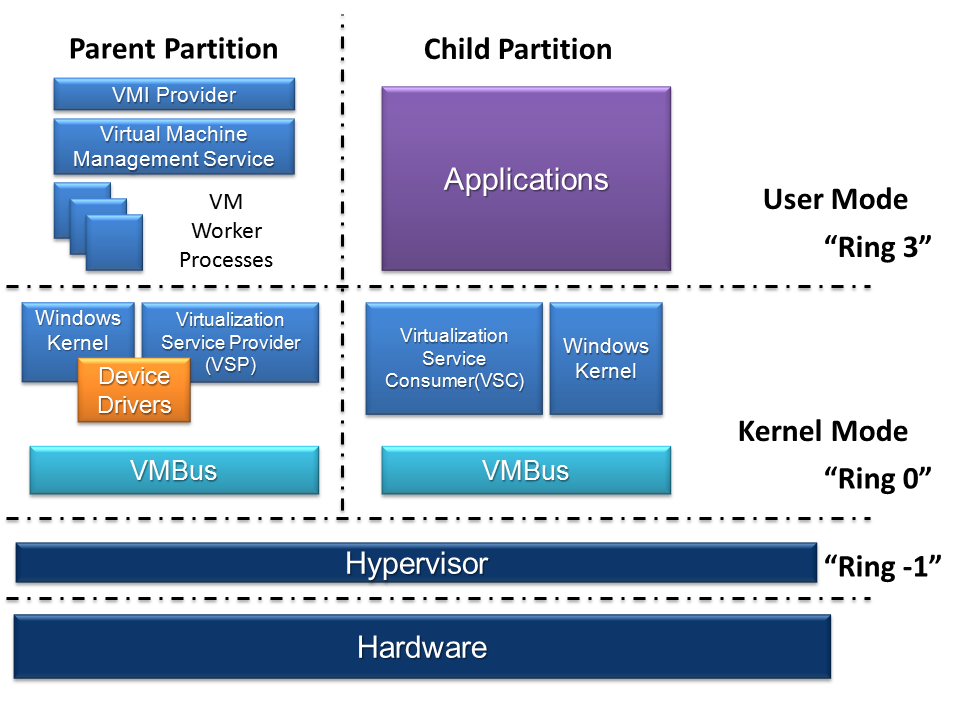
\includegraphics[width=\linewidth]{images/arch}}
\caption{Hyper-V architechture \cite{www-hyperv-wikipedia}.}
\label{fig:false-color}
\end{figure}

\section{Prerequisites}

To install Hyper-V we need to have an x64 based processor with a
minimum of 1.4GHz clock speed. We also need to enable
hardware-assisted virtualization, this feature is available in
processors that include an inbuilt virtualization option specifically,
Intel Virtualization Technology or AMD Virtualization. It also
requires hardware-enforced Data Execution Prevention
(DEP). Specifically, Intel XD bit (execute disable bit) or AMD NX bit
(no execute bit)must be enabled \cite{www-hyperv-paper2}. The
processor should also support second level address
translation. Minimum 2 GB memory with error correcting code or similar
technology is required, realistically much more memory is required as
each virtual machine requires its own memory. The installation also
requires a minimum of 32GB disk space. Apart from the above mentioned
requirements, there are other requirements which are not mandatory but
required to enable certain features \cite{www-hyperv-wikipedia}.

\section{Installation}

Installation of Hyper-V needs you to install Windows Server 2012 R2,
for which you need a bootable device having the same and boot the
device using it. Select the operating system you need to install
i.e. standard/datacenter.  Accept the terms and select install windows
and select the drive you want to install the operating system on, we
need a minimum of 32GB space for the installation. Set the username
and password and then login. After logging on change the host name by
going under my computer system properties. Open the server manager and
configure according to the requirements which include selecting the
roles and feature as required. Select the server name and click next
and wait for the installation to complete
\cite{www-hyperv-paper2}. Once Hyper-V is installed you can install
create virtual networks and create virtual machines on which you can
then install the operating system.

\section{Advantages and Features}

With Windows Server 2012, Hyper-V supports network virtualization,
multi-tenancy, vhdx disk format supporting virtual hard disks as
large as 64TB, offloaded data transfer, cross-premises connectivity
and Hyper-V replica. And with Windows Server 2012 R2 also supports
shared virtual hard disk, storage quality of services, enhances
session mode \cite{www-hyperv-wikipedia}. Multiple physical servers
can be easily consolidated into comparatively fewer servers by
implementing virtualization with Hyper-V. Consolidation accommodates
the full use of deployed hardware resources. Hyper-V also helps in
ease of administration as consolidation and centralization of
resources simplifies administration and scale-up or scale-out can be
accommodated with much greater ease. With Hyper-V and with
virtualization, in general, there are significant cost savings. As
separate physical machines are not required for every host and
multiple virtual machines can be easily setup on a single physical
machine. Hyper-V can be easily managed and a comprehensive Hyper-V
management solution is available with System Center Virtual Machine
Manager.  Additional processing power, network bandwidth, and storage
capacity can be accomplished quickly and easily by assigning
additional resources from the host computer to the guest virtual
machinws \cite{www-hyperv-advantages}.

\section{Limitations}

Hyper-V does not virtualize audio hardware. It does not support the
host/root operating system's optical drives to pass-through guest VMs,
as a result, burning to disks are not supported. In Windows Server
2008, Hyper-V does not support live migration of guest VMs where live
migration is maintaining network connections and uninterrupted
services during VM migration between physical hosts. Although Hyper-V
doesn't provide live migration but it tries to eliminate the
limitation by having quick migration feature. Also, when Hyper-V is
installed it uses VT-x x86 virtualization feature making it
unavailable for other solutions due to which software which requires
VT-x support can't be installed in parallel
\cite{www-hyperv-wikipedia}. One of the major operating system that is
still unsupported includes Fedora 8 and 9 \cite{www-hyperv-wikipedia}.

\section{Management}

Hyper-V servers can be managed using Windows PowerShell either locally
or remotely \cite{www-microsoft-technet}. By running server manager on
a remote computer, a server running in server core mode can be
connected. It can also be connected using Microsoft Management Console
(MMC) snap-in or by using another computer running Windows, the user
can use Remote Desktop Services to run scripts and tools on a server
\cite{www-microsoft-technet}. Server can be switched to graphical user
interface mode to use the usual user interface tools to accomplish the
tasks and then switch back to server core mode
\cite{www-microsoft-technet}.

Hype-V hosts can be managed using Hyper-V manager where the manager
lets you manage a small number of Hyper-V hosts, both remote and
local. It's gets installed with the installation of Hyper-V Management
Tools, which can be installed through a full Hyper-V installation or a
tools-only installation \cite{www-microsoft-technet}.

\section{Comparison between Hyper-V and vSphere}

Windows Server 2012 R2, VMware vSphere Hypervisor and VMware vSphere
5.5 Enterprise Plus all support 320 logical processors, 4TB of
physical memory, 1TB of memory per virtual machine. While Hyper-V and
vSphere Enterprise edition both support 64 virtual CPUs per virtual
machine, vSphere Hypervisor only support 8. In Hyper-V there can be
1,024 active VMs per host while this is limited to 512 in vSphere. It
is interesting to know that Hyper-V supports up to 64 nodes and up to
8,000 virtual machines per in a cluster while vShere Enterprise plus
supports 32 and 4,000 respectively \cite{www-hyperv-paper}.

Both VMware vSphere Hypervisor and Hyper-V are free standalone
hypervisors, however enterprise edition of vSphere is not. The above
information shows that Hyper-V has a number of advantages from a
scalability perspective, especially when it comes to comparison with
the vSphere Hypervisor \cite{www-hyperv-paper}. VMware vSphere 5.5
brought a number of scalability increases for vSphere environments,
doubling the number of host logical processors supported from 160 to
320, and doubling the host physical memory from 2TB to 4TB, but this
still only brings vSphere up to the level that Hyper- V has been
offering since September 2012 \cite{www-hyperv-paper}. Hyper-V also
supports double the number of active virtual machines per host, than
both the vSphere Hypervisor and vSphere 5.5 Enterprise Plus.


\section{Conclusion}

Hyper-V is a powerful hypervisor introduced by Microsoft with features
such as high availability, scalability, reliability, flexibility. It
also supports resource monitoring that helps user track historical
data on the use of virtual machines and gain insight into the resource
use of specific servers. Hyper-V sees competition from many other
supervisors such as vSphere, Qemu, KVM, VirtualBox and provides a
tough competition. Hyper-V requires hardware assisted virtualization
support from processors and it can only be used with x86-64
processors. In spite of it's limitations it's a popular choice because
of the features it provides. The customization options available in
Hyper-V provides the user with lot of options to manage the virtual
machines as he would like. Hyper-V and Hyper-V hosts can be easily
managed using Windows PowerShell and Hyper-V manager tool locally or
remotely.

% Bibliography

\bibliography{references}

\end{document}
\grid
